\documentclass[10pt,letterpaper]{article} 
\usepackage[margin=1in]{geometry}
\usepackage[utf8]{inputenc}
\usepackage[spanish,english]{babel}

\usepackage{amsmath}
\usepackage{amsfonts}
\usepackage{amssymb}
\usepackage{physics}
\usepackage{bbm}

\usepackage{graphicx}
\graphicspath{{../figs/}}

\usepackage[dvipsnames]{xcolor}

\usepackage{float}

\newcommand{\eref}[1]{eq.~(\ref{#1})} 
\newcommand{\sref}[1]{sec.~\ref{#1}}
\newcommand{\fref}[1]{Fig.~\ref{#1}}
\newcommand{\tref}[1]{table~\ref{#1}}
\newcommand{\Eref}[1]{Eq.~(\ref{#1})} 
\newcommand{\Sref}[1]{Sec.~\ref{#1}}
\newcommand{\Fref}[1]{Fig.~\ref{#1}}  
\newcommand{\Tref}[1]{Table~\ref{#1}}

\usepackage{hyperref}
\hypersetup{
colorlinks=true,
linkcolor=blue,
filecolor=blue,      
citecolor=blue,
urlcolor=blue,
pdftitle={},
pdfauthor=author={Jose Alfredo de Leon},
}

\usepackage{tikz}

\usepackage[mathlines]{lineno}  \linenumbers \setlength\linenumbersep{5pt}
\usepackage[inline]{showlabels,rotating}
\renewcommand{\showlabelrefline}{\hrule width 0pt height 3ex depth 0pt}
\renewcommand{\showlabelfont}{\small\slshape\color{red!70}}
\usepackage[draft,inline,nomargin]{fixme} \fxsetup{theme=color}
\definecolor{jacolor}{RGB}{200,40,0} \FXRegisterAuthor{ja}{aja}{\color{jacolor}JA}
\FXRegisterAuthor{cp}{acp}{\color{blue}CP}
\FXRegisterAuthor{cd}{acd}{\color{purple}CD}

\decimalpoint

\newcommand{\one}{\mathbbm{1}}

\title{Quantum chaos meets quantum channels}
\author{}
\date{\today}

\renewcommand{\labelenumii}{\arabic{enumi}.\arabic{enumii}}
\renewcommand{\labelenumiii}{\arabic{enumi}.\arabic{enumii}.\arabic{enumiii}}
\renewcommand{\labelenumiv}{\arabic{enumi}.\arabic{enumii}.\arabic{enumiii}.\arabic{enumiv}}

% --------------------------------------------------------------------------------------------------
% Comamands for this document
\newcommand{\mcE}{\mathcal E}
\newcommand{\mcP}{\mathcal P}
% --------------------------------------------------------------------------------------------------

\begin{document}
\maketitle

%\section{Ideas}
%The evolution of the chaometer qubit can be understood as a quantum channel:
%\begin{align}
%\rho_1(t) = 
%\mcE[\rho_1(0)] = 
%\Tr_E\qty(e^{-iHt} \rho_1(0)\otimes \rho_E(0) e^{-iHt}),
%\end{align}
%where $\rho_1(0) \otimes \rho_E(0) = \dyad{\psi(0)}$, 
%with $\ket{\psi(0)}$ is a $L$-qubit random product state; and $H$ the spin chain 
%Hamiltonian.
%
%The quantum channel $\mcE$ can be written in its Kraus form:
%\begin{align}
%\mcE(\rho_1) = 
%\sum_{i=1}^{r\leq 4} K_i \rho_1 K_j^\dagger,
%\end{align}
%with $r$ is the Kraus rank of $\mcE$.
%
%The purity $\mcP$ of the chaometer now reads:
%\begin{align}
%\mcP [\mcE(\rho_1)] &=
%\Tr \big\{\qty[\mcE(\rho_1)]^2 \big\}\\
%&= \sum_{i,j=1}^{r\leq 4}
%\Tr \qty( K_i \rho K_i^\dagger K_j \rho K_j^\dagger) \\
%&= \sum_{i,j}^{r\leq 4}
%\Tr \qty( K_j^\dagger K_i \rho K_i^\dagger K_j \rho).
%\end{align}
%My guess is that the chaotic information of the system has to be 
%encoded in operators $K_i^\dagger K_j$. To further explore this idea 
%I will examine the relationship $\mcP [\mcE(\rho_1)]  = 1 - \eta $.
%
%Integrable:
%\begin{align}
%\mcP [\mcE(\rho_1)] = 
%\min \qty[
%\frac{1}{N} \sum_{i=1}^N 
%\qty(\frac{1}{T}\int_0^T 
%\Tr [\rho_i^2(t)] dt
%)
%] \approx 1
%\end{align}
%
%Chaotic:
%\begin{align}
%\mcP [\mcE(\rho_1)] = 
%\max \qty[
%\frac{1}{N} \sum_{i=1}^N 
%\qty(\frac{1}{T}\int_0^T 
%\Tr [\rho_i^2(t)] dt
%)
%] \approx \frac{1}{2}
%\end{align}

\section{Model}
The spin chain we are interested in studying first is that studied by 
Mirkin and Wisniacki in Ref.~\cite{mirkin2021quantum}:
\begin{equation}\label{eq:H:wisniacki:ising:chain}
H = 
\sum_{i=1}^{L}
\qty(
h_x \sigma_i^x +
h_z \sigma_i^z
) -
\sum_{i=1}^{L-1}
J_z \sigma_{i}^z \sigma_{i+1}^z.
\end{equation}

\section{Mean level spacing ratio}
The level spacing ratio $\tilde r_n$ is defined as:
\begin{equation}\label{eq:level:spacing:ratio}
\tilde r_n= 
\frac{\min(s_n, s_{n-1})}{\max(s_n, s_{n-1})}, 
\end{equation}
where $s_n = E_{n+1} - E_n$. The mean level spacing ratio $\expval{\tilde r_n}$ is 
known to attain the value $\expval{\tilde r_n} \approx 0.5207$ when the 
level spacing distribution $P(s)$ is Wigner-Dyson and
$\expval{\tilde r_n} \approx 0.386$ when it is Poisson.

\begin{figure}
\centering
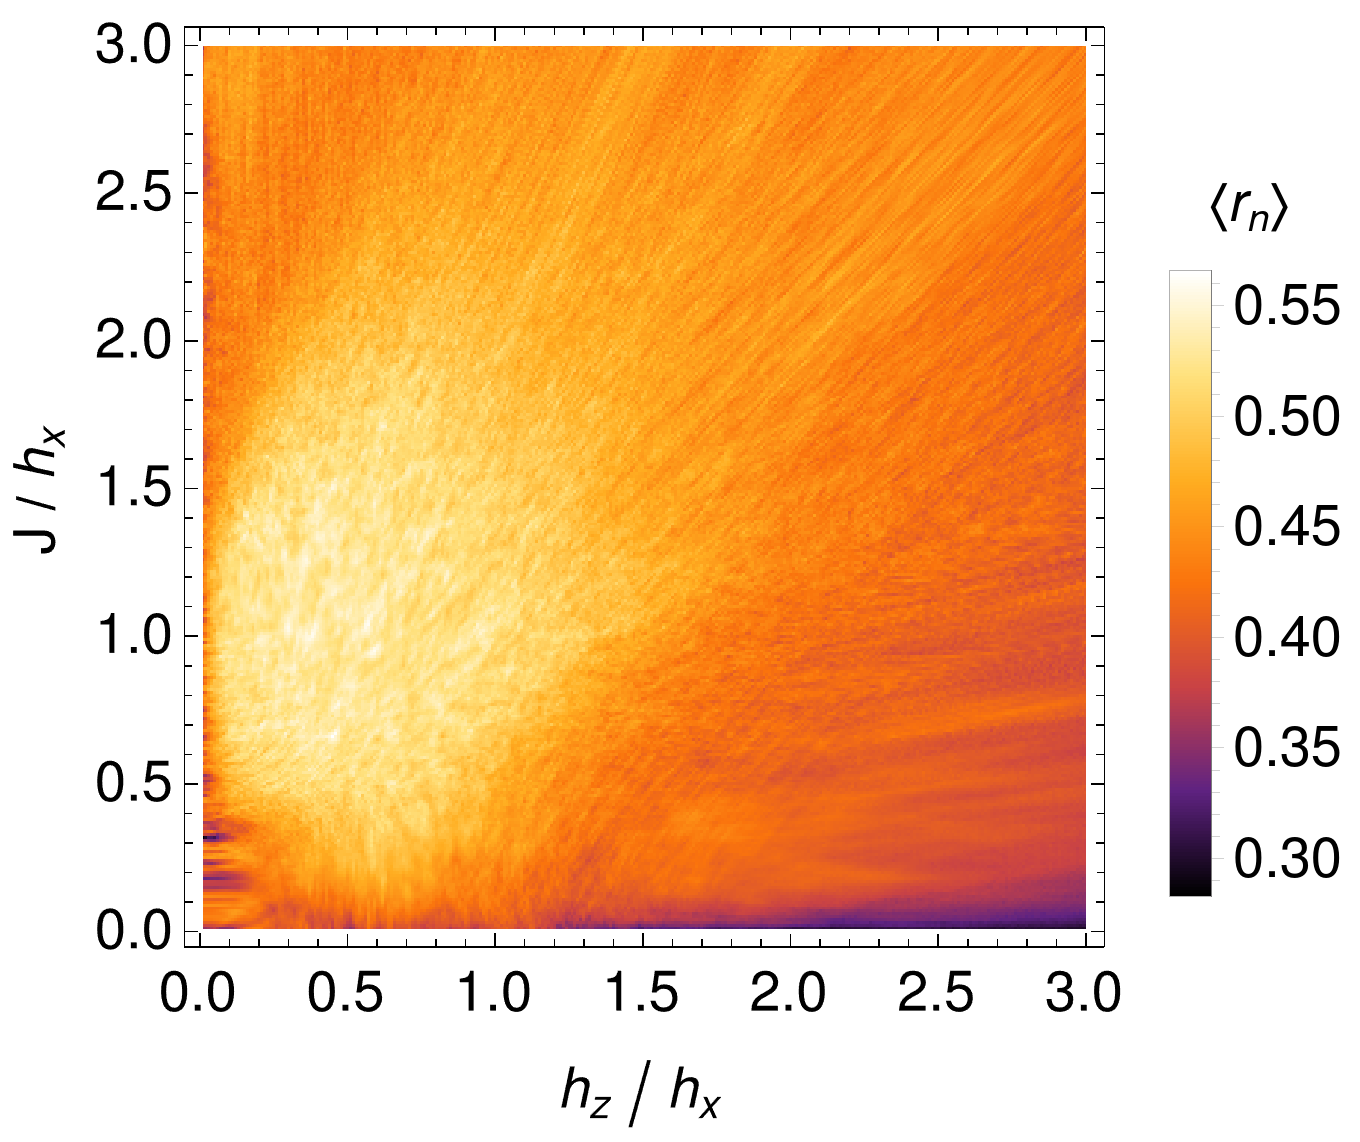
\includegraphics[width=0.7\textwidth]{mean_level_spacing_ratio.png}
\caption{Mean level spacing ratio $\expval{\tilde r_n}$ 
[c.f.~\eref{eq:level:spacing:ratio}] of the Ising chain 
with Hamiltonian \eqref{eq:H:wisniacki:ising:chain} as a function of ratios 
$h_z/h_x$ and $J/h_x$. We assume $J_z=J\, \forall\,k$.}
\label{fig:mean:level:spacing:ratio}
\end{figure}

\section{Spectral form factor}
The spectral form factor $K(t)$ is defined as:
\begin{equation}\label{eq:sff}
K(t) = 
\frac{1}{2^L}
\expval{
\abs{\Tr U(t) }^2
} = 
\frac{1}{2^L}
\expval{
\sum_{i,j} 
e^{i(E_i - E_j) t}
},
\end{equation}
\begin{figure}
\centering
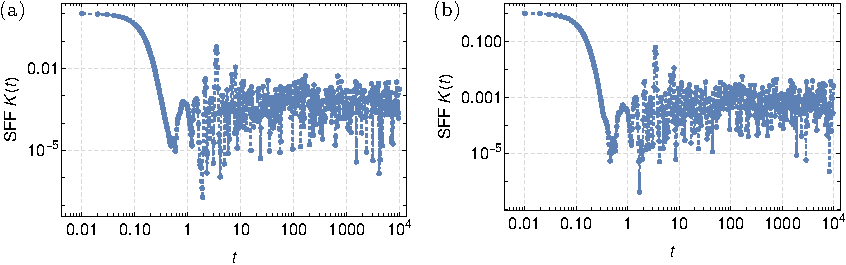
\includegraphics[width=\textwidth]{sff_regular.pdf}
\caption{Spectral form factor (SFF) [c.f.~\eqref{eq:sff}] in regular region: $h_z/h_x=2.5$ and 
$J/h_x=1$. \textbf{(a)} Whole spectrum. \textbf{(b)}~Even-parity subspace 
spectrum.}
\label{fig:sff:regular}
\end{figure}
where $\expval{\cdot}$ denotes the ensemble-average over statistically-similar
systems.

\begin{figure}
\centering
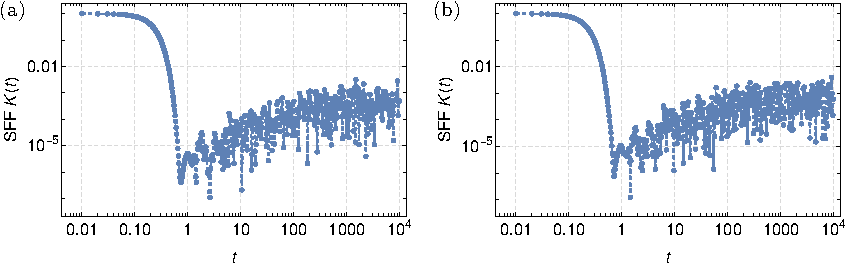
\includegraphics[width=\textwidth]{sff_chaotic.pdf}
\caption{Spectral form factor (SFF) [c.f.~\eqref{eq:sff}] in chaotic region: $h_z/h_x=0.5$ and 
$J/h_x=1$. \textbf{(a)} Whole spectrum. \textbf{(b)}~Even-parity subspace 
spectrum.}
\label{fig:sff:chaotic}
\end{figure}

\section{Chaometer's quantum channel}
The reduced dyanmics of the chaometer is described by the quantum channel: 
\begin{equation}
\mcE(\rho) = 
\Tr_E \qty(
e^{-i H t}
\rho \otimes \dyad{\psi_0^{(E)}}
e^{i H t}
),
\end{equation}
where $H$ is that of~\eref{eq:H:wisniacki:ising:chain}, $\ket{\psi_0^{(E)}}$
the initial state of all spins except the chaometer, and $\rho$ the initial 
state of the chaometer. 

The chaometer's quantum channel $\mcE$, in general, is divisible into: 
\begin{enumerate}
\item A unitary operation rotating the Bloch's sphere.
\item A quantum channel that deforms the Bloch's sphere and translates its origin.
\end{enumerate}
Both operations do not commute. 

\bibliographystyle{unsrt}
\bibliography{references.bib}

\end{document}